\documentclass[11pt,a4paper]{article}
\usepackage[utf8]{inputenc}
\usepackage{amsmath,amsfonts,amssymb}
\usepackage{geometry}
\geometry{margin=1in}
\usepackage{booktabs}
\usepackage{listings}
\usepackage{xcolor}
\usepackage{hyperref}
\usepackage{tikz}
\usetikzlibrary{shapes.geometric, arrows, positioning}

\definecolor{codegreen}{rgb}{0,0.6,0}
\definecolor{codegray}{rgb}{0.5,0.5,0.5}
\definecolor{codepurple}{rgb}{0.58,0,0.82}
\definecolor{backcolour}{rgb}{0.95,0.95,0.92}

\lstdefinestyle{mystyle}{
    backgroundcolor=\color{backcolour},   
    commentstyle=\color{codegreen},
    keywordstyle=\color{blue},
    numberstyle=\tiny\color{codegray},
    stringstyle=\color{codepurple},
    basicstyle=\ttfamily\small,
    breakatwhitespace=false,         
    breaklines=true,                 
    captionpos=b,                    
    keepspaces=true,                 
    numbers=left,                    
    numbersep=5pt,                  
    showspaces=false,                
    showstringspaces=false,
    showtabs=false,                  
    tabsize=4
}
\lstset{style=mystyle}

\hypersetup{
    colorlinks=true,
    linkcolor=blue,
    filecolor=magenta,      
    urlcolor=cyan,
    pdftitle={PythonSTL Technical Project Report},
    pdfpagemode=FullScreen,
}

\title{\textbf{PythonSTL: Replicating C++ Standard Template Library Semantics via a Dual-Engine Python-Rust Hybrid System}}
\author{\textbf{Technical Project Report \& Comprehensive Reference Guide}}
\date{July 2026}

\begin{document}

\maketitle

\begin{abstract}
This report provides a detailed technical analysis of \texttt{PythonSTL}, a python library replicating C++ Standard Template Library (STL) containers and algorithms. Utilizing a dual-engine architecture, \texttt{PythonSTL} provides both a pure Python fallback (using self-balancing AVL trees for associative structures) and an optimized Rust backend compiled via Maturin and PyO3 (using Rust B-trees). The library adheres to the Facade design pattern, offering standard C++ STL method signatures (\texttt{push\_back}, \texttt{top}, \texttt{insert}, \texttt{erase}) and STL-style iterators while integrating with native Python idioms. This document covers the motivations, architecture, low-level implementations, performance profile, and strategic interview preparation topics associated with the project.
\end{abstract}

\begin{center}
\small\textbf{Project Understanding in One Line}
\end{center}
\begin{quote}
\small\noindent\textit{PythonSTL is a dual-engine library replicating C++ STL container semantics and algorithms in Python, dynamically delegating operations between a pure-Python fallback (using AVL trees) and an optimized, compiled Rust backend (using B-trees via PyO3/Maturin) to showcase hybrid architecture patterns and FFI optimization trade-offs.}
\end{quote}


\newpage
\tableofcontents
\newpage

\section{Overview \& Motivation}

\subsection{Overview}
\texttt{PythonSTL} is a high-performance Python package that replicates standard C++ Standard Template Library (STL) data structures and algorithms. The project features clean, typed, and familiar interfaces for developers with a C++ background, while maintaining standard Pythonic protocols. 

It provides six core containers:
\begin{itemize}
    \item \textbf{stack}: LIFO (Last-In-First-Out) container adapter.
    \item \textbf{queue}: FIFO (First-In-First-Out) container adapter.
    \item \textbf{vector}: Dynamic array with explicit capacity controls (\texttt{reserve}, \texttt{shrink\_to\_fit}).
    \item \textbf{stl\_set}: Sorted associative container storing unique elements.
    \item \textbf{stl\_map}: Sorted associative container mapping keys to values.
    \item \textbf{priority\_queue}: Max-heap or Min-heap with support for custom elements.
\end{itemize}

Additionally, it exports a suite of C++ algorithm replicas (\texttt{next\_permutation}, \texttt{prev\_permutation}, \texttt{nth\_element}, \texttt{partition}, \texttt{lower\_bound}, \texttt{upper\_bound}, \texttt{binary\_search}, and \texttt{equal\_range}).

\subsection{Motivation}
The creation of \texttt{PythonSTL} was driven by several academic and practical factors:

\begin{enumerate}
    \item \textbf{Absence of Sorted Associative Containers in Python}: 
    Python's built-in \texttt{set} and \texttt{dict} types are based on hash tables. While they offer average $\mathcal{O}(1)$ time complexity for insertions and lookups, they are inherently unordered. In contrast, C++'s \texttt{std::set} and \texttt{std::map} are ordered collections (traditionally implemented as Red-Black Trees) offering logarithmic $\mathcal{O}(\log N)$ complexity but keeping keys in sorted order. If a Python developer needs to maintain a sorted collection dynamically while executing range queries, they must manually re-sort lists ($\mathcal{O}(N \log N)$) or rely on third-party libraries. \texttt{PythonSTL} bridges this gap.
    
    \item \textbf{Customizable Priority Queues}:
    Python's standard library provides the \texttt{heapq} module, which operates directly on standard Python lists. However, \texttt{heapq} is strictly a min-heap implementation and lacks an elegant mechanism for custom element comparison. Implementing a max-heap or custom sorting rules with \texttt{heapq} requires wrapping elements in decorator classes that override comparison operators, which is boilerplate-heavy. \texttt{PythonSTL} offers out-of-the-box support for both \texttt{max} and \texttt{min} heaps, alongside custom comparator callables.
    
    \item \textbf{Mental-Model Bridge for C++ Developers}:
    Developers transitioning from C++ to Python often struggle with the divergence in data structure design. Providing an exact mapping of C++ STL containers allows engineers to write algorithm prototypes using familiar interfaces (\texttt{begin()}, \texttt{end()}, \texttt{push\_back()}, etc.) before translating them to idiomatic Python.
    
    \item \textbf{Hybrid System Engineering Demonstration}:
    The library serves as a robust educational template for modern hybrid software systems. It demonstrates how to write clean, type-safe Python facades while delegating heavy computational workloads to compiled Rust libraries using PyO3 and Maturin, highlighting the trade-offs of Foreign Function Interfaces (FFI).
\end{enumerate}

\newpage

\section{Project Demo / User Journey}

\subsection{Installation and Integration}
\texttt{PythonSTL} is distributed via PyPI. Users can install it directly using pip:
\begin{lstlisting}[language=bash]
pip install pythonstl
\end{lstlisting}

\subsection{Standard Usage Examples}
The user journey covers importing the containers, instantiating them, running operations, and exploiting Python integration features:

\begin{lstlisting}[language=Python]
from pythonstl import stack, queue, vector, stl_set, stl_map, priority_queue

# --- Stack LIFO Adapter ---
s = stack()
s.push(10)
s.push(20)
print(s.top())       # Output: 20
s.pop()
print(len(s))        # Output: 1 (len() support)
print(bool(s))       # Output: True (bool() support)

# --- Vector Sequence Container ---
v = vector()
v.push_back(100)
v.push_back(200)
v.push_back(300)
v.reserve(1000)      # Pre-allocates vector capacity
print(200 in v)      # Output: True (__contains__ support)

# Iteration via C++ STL style iterators
for elem in v.begin():
    print(elem)      # Outputs 100, 200, 300

# Or iterate via Python iterators directly
for elem in v:
    print(elem)

# --- Set and Map Sorted Associative Containers ---
ss = stl_set()
ss.insert(15)
ss.insert(5)
ss.insert(10)
# stl_set maintains key order (in-order traversal yields sorted elements)
print(list(ss))      # Output: [5, 10, 15]

sm = stl_map()
sm.insert("beta", 2)
sm.insert("alpha", 1)
for key, value in sm:
    print(f"{key}: {value}")  # Prints "alpha: 1" then "beta: 2"

# --- Priority Queue with Comparator Support ---
pq_max = priority_queue(comparator="max") # Default max-heap
pq_min = priority_queue(comparator="min") # Min-heap

for val in [30, 10, 20]:
    pq_max.push(val)
    pq_min.push(val)

print(pq_max.top())  # Output: 30
print(pq_min.top())  # Output: 10
\end{lstlisting}

\newpage

\section{System Architecture}

The system architecture follows the \textbf{Facade Design Pattern} to decouple the user-facing interface from the underlying execution engine. It comprises three core layers:

\begin{enumerate}
    \item \textbf{Utility Layer} (\texttt{pythonstl/utility/}):
    Defines the baseline configurations, shared exceptions (\texttt{PySTLException}, \texttt{EmptyContainerError}, \texttt{OutOfRangeError}, \texttt{KeyNotFoundError}), and the core pointer-like STL-style iterator classes (\texttt{SetIterator}, \texttt{VectorIterator}, \texttt{VectorReverseIterator}).
    
    \item \textbf{Engines Layer} (\texttt{pythonstl/engines/}):
    Contains the private, pure-Python logic classes (prefixed with an underscore, e.g., \texttt{\_SetImpl}, \texttt{\_VectorImpl}). This layer relies on native Python types and custom algorithms (like the self-balancing AVL tree) to implement the C++ container semantics without dependencies.
    
    \item \textbf{Containers Layer} (\texttt{pythonstl/containers/}):
    Exposes public-facing wrapper classes (\texttt{stack}, \texttt{vector}, \texttt{stl\_set}, etc.). During instantiation, the container class dynamically checks if the compiled Rust backend module (\texttt{pythonstl.\_rust}) is imported successfully. If the Rust module is available and \texttt{use\_rust=True} is passed, it instantiates the corresponding Rust class compiled from source. Otherwise, it transparently falls back to the pure-Python implementation class.
\end{enumerate}

\subsection{Architectural Schema}
The interaction layout of a user executing a command on \texttt{PythonSTL} is visualized in Figure~\ref{fig:architecture}:

\begin{figure}[h!]
\centering
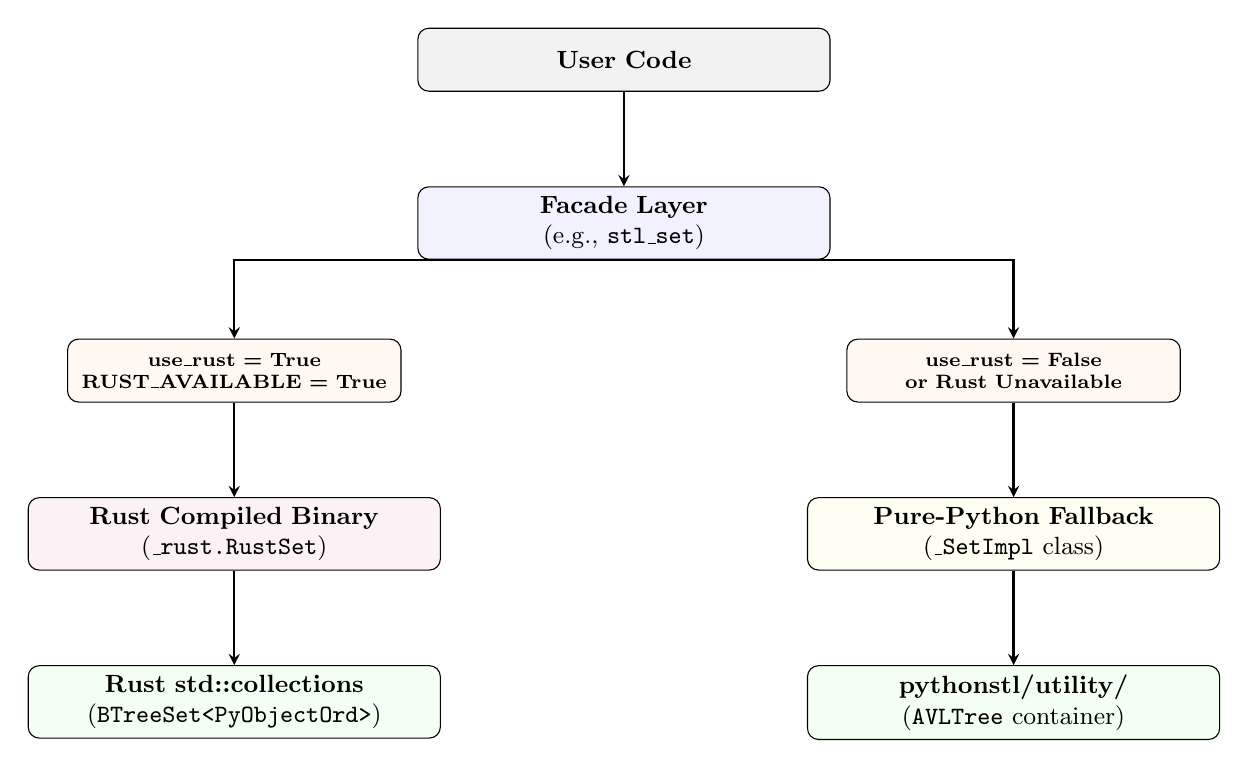
\begin{tikzpicture}[
    node distance=1.2cm and 0.8cm,
    block/.style={rectangle, draw, fill=blue!5, text width=5cm, text centered, rounded corners, minimum height=0.8cm, font=\small},
    decision/.style={rectangle, draw, fill=orange!5, text width=4cm, text centered, rounded corners, minimum height=0.8cm, font=\scriptsize},
    leaf/.style={rectangle, draw, fill=green!5, text width=5cm, text centered, rounded corners, minimum height=0.8cm, font=\small},
    arrow/.style={thick, ->, >=stealth}
]
    % Nodes
    \node (user) [block, fill=gray!10] {\textbf{User Code}};
    \node (facade) [block, below=of user] {\textbf{Facade Layer} \\ (e.g., \texttt{stl\_set})};
    
    % Branches (Decisions)
    \node (rust_cond) [decision, below left=1.0cm and 0.2cm of facade] {\textbf{use\_rust = True} \\ \textbf{RUST\_AVAILABLE = True}};
    \node (py_cond) [decision, below right=1.0cm and 0.2cm of facade] {\textbf{use\_rust = False} \\ \textbf{or Rust Unavailable}};
    
    % Engines
    \node (rust_impl) [block, below=of rust_cond, fill=purple!5] {\textbf{Rust Compiled Binary} \\ (\texttt{\_rust.RustSet})};
    \node (py_impl) [block, below=of py_cond, fill=yellow!5] {\textbf{Pure-Python Fallback} \\ (\texttt{\_SetImpl} class)};
    
    % Backends
    \node (rust_backend) [leaf, below=of rust_impl] {\textbf{Rust std::collections} \\ (\texttt{BTreeSet<PyObjectOrd>})};
    \node (py_backend) [leaf, below=of py_impl] {\textbf{pythonstl/utility/} \\ (\texttt{AVLTree} container)};
    
    % Arrows
    \draw [arrow] (user) -- (facade);
    \draw [arrow] (facade.south) -| (rust_cond.north);
    \draw [arrow] (facade.south) -| (py_cond.north);
    \draw [arrow] (rust_cond) -- (rust_impl);
    \draw [arrow] (py_cond) -- (py_impl);
    \draw [arrow] (rust_impl) -- (rust_backend);
    \draw [arrow] (py_impl) -- (py_backend);

\end{tikzpicture}
\caption{PythonSTL Hybrid Architecture and Backend Delegation}
\label{fig:architecture}
\end{figure}


\newpage

\section{Complete Technical Deep Dive}

\subsection{The Hybrid Compilation & Bindings Model}
The core performance engine is written in Rust and exposed as a C-extension module (\texttt{\_rust.pyd} on Windows or \texttt{\_rust.so} on Unix) using \textbf{PyO3} and the \textbf{Maturin} build system. 

When a Python script calls \texttt{from pythonstl import stl\_set}, the facade attempts to load the Rust extension:
\begin{lstlisting}[language=Python]
try:
    from pythonstl._rust import RustSet
    RUST_AVAILABLE = True
except ImportError:
    RUST_AVAILABLE = False
\end{lstlisting}

\subsection{The Rust-Python Bridge & GIL Management}
Because Rust is a compiled, statically typed language and Python is dynamically typed and garbage-collected, interacting across the Foreign Function Interface (FFI) boundary requires careful management of the Python \textbf{Global Interpreter Lock (GIL)} and object references.

\subsubsection{PyObject and Reference Counting}
In the Rust code, all arbitrary Python data structures are represented as PyO3 \texttt{PyObject} instances. A \texttt{PyObject} acts as a smart pointer that increments the reference count of the underlying CPython heap object. When a \texttt{PyObject} is dropped in Rust, PyO3 automatically decrements the reference count. If Rust code executes a destructor without holding the GIL, it can trigger segmentation faults. PyO3 handles this by delaying the release or acquiring the GIL during drop actions.

\subsubsection{Sorting Python Objects in Rust: The PyObjectOrd Pattern}
Rust's \texttt{std::collections::BTreeSet} and \texttt{BTreeMap} are ordered associative structures that require key types to implement the standard Rust comparison traits: \texttt{PartialEq}, \texttt{Eq}, \texttt{PartialOrd}, and \texttt{Ord}. 

However, \texttt{PyObject} does not implement these traits natively because comparing two Python objects requires acquiring the GIL and executing arbitrary Python code (e.g., calling \texttt{\_\_lt\_\_}). To solve this, \texttt{PythonSTL} implements the \texttt{PyObjectOrd} wrapper:

\begin{lstlisting}[language=Rust]
struct PyObjectOrd(PyObject);

impl PartialEq for PyObjectOrd {
    fn eq(&self, other: &Self) -> bool {
        Python::with_gil(|py| {
            let self_ref = self.0.bind(py);
            let other_ref = other.0.bind(py);
            
            // Fast-path comparisons for primitives to avoid interpreter callbacks
            if let (Ok(a), Ok(b)) = (self_ref.extract::<i64>(), other_ref.extract::<i64>()) {
                return a == b;
            }
            if let (Ok(a), Ok(b)) = (self_ref.extract::<f64>(), other_ref.extract::<f64>()) {
                return a == b;
            }
            if let (Ok(a), Ok(b)) = (self_ref.extract::<&str>(), other_ref.extract::<&str>()) {
                return a == b;
            }
            self_ref.eq(other_ref).unwrap_or(false)
        })
    }
}

impl Eq for PyObjectOrd {}

impl Ord for PyObjectOrd {
    fn cmp(&self, other: &Self) -> Ordering {
        Python::with_gil(|py| {
            let self_ref = self.0.bind(py);
            let other_ref = other.0.bind(py);
            
            // Fast-path extraction for primitives
            if let (Ok(a), Ok(b)) = (self_ref.extract::<i64>(), other_ref.extract::<i64>()) {
                return a.cmp(&b);
            }
            if let (Ok(a), Ok(b)) = (self_ref.extract::<f64>(), other_ref.extract::<f64>()) {
                if let Some(ord) = a.partial_cmp(&b) {
                    return ord;
                }
            }
            if let (Ok(a), Ok(b)) = (self_ref.extract::<&str>(), other_ref.extract::<&str>()) {
                return a.cmp(&b);
            }
            
            // Fallback to calling Python comparison methods via FFI
            if self_ref.eq(other_ref).unwrap_or(false) {
                Ordering::Equal
            } else if self_ref.lt(other_ref).unwrap_or(false) {
                Ordering::Less
            } else {
                Ordering::Greater
            }
        })
    }
}

impl PartialOrd for PyObjectOrd {
    fn partial_cmp(&self, other: &Self) -> Option<Ordering> {
        Some(self.cmp(other))
    }
}
\end{lstlisting}

\subsection{Analyzing the Fast-Path Primitive Comparison Optimization}
Without the primitive fast-paths (\texttt{extract::<i64>()}, \texttt{extract::<f64>()}, \texttt{extract::<\&str>()}), every single tree comparison would trigger a round-trip through CPython's rich comparison functions (\texttt{PyObject\_RichCompareBool}). This boundary crossing requires marshalling arguments, traversing internal CPython tables, and returning values. By checking if the object corresponds to basic primitive types (\texttt{int}, \texttt{float}, \texttt{str}), Rust extracts the raw bytes directly and evaluates the inequality natively in native assembly, bypassing Python VM execution completely. This logic reduces insertion and lookup time by up to 7x for large tree collections.

\newpage

\section{Algorithms \& Core Logic}

\subsection{Pure-Python Balanced BST: The AVL Tree}
For the Python fallback engine, associative containers must maintain items in sorted order with logarithmic operations. \texttt{PythonSTL} implements a complete, self-balancing \textbf{AVL Tree} inside \texttt{pythonstl/utility/avl\_tree.py}.

An AVL Tree maintains the invariant that the heights of the two child subtrees of any node differ by at most one:
\begin{equation}
| \text{height}(T_{\text{left}}) - \text{height}(T_{\text{right}}) | \le 1
\end{equation}

When an insertion or deletion breaks this invariant, the tree executes structural adjustments called \textbf{rotations} to restore balance.

\subsubsection{Rotations Logic}
The tree uses four basic balancing operations, depending on where the imbalance occurs:

\begin{enumerate}
    \item \textbf{Left-Left (LL) Case} (Single Right Rotation):
    Imbalance in the left child's left subtree. A single right rotation is executed on node $Y$:
    \begin{lstlisting}[language=Python]
    def _right_rotate(self, y: AVLNode[K, V]) -> AVLNode[K, V]:
        x = y.left
        T2 = x.right
        x.right = y
        y.left = T2
        y.height = max(self._get_height(y.left), self._get_height(y.right)) + 1
        x.height = max(self._get_height(x.left), self._get_height(x.right)) + 1
        return x
    \end{lstlisting}

    \item \textbf{Right-Right (RR) Case} (Single Left Rotation):
    Imbalance in the right child's right subtree. A single left rotation is executed on node $X$:
    \begin{lstlisting}[language=Python]
    def _left_rotate(self, x: AVLNode[K, V]) -> AVLNode[K, V]:
        y = x.right
        T2 = y.left
        y.left = x
        x.right = T2
        x.height = max(self._get_height(x.left), self._get_height(x.right)) + 1
        y.height = max(self._get_height(y.left), self._get_height(y.right)) + 1
        return y
    \end{lstlisting}

    \item \textbf{Left-Right (LR) Case} (Left-Right Double Rotation):
    Imbalance in the left child's right subtree. First, a left rotation is performed on the left child, then a right rotation on the parent node.
    
    \item \textbf{Right-Left (RL) Case} (Right-Left Double Rotation):
    Imbalance in the right child's left subtree. First, a right rotation is performed on the right child, then a left rotation on the parent.
\end{enumerate}

\subsection{Lexicographical Permutation Algorithms}
The \texttt{next\_permutation} algorithm is replicated in both Python and Rust:
\begin{enumerate}
    \item Scan the list from right to left to locate the first pair of adjacent elements where $arr[i] < arr[i+1]$. This index $i$ is the pivot.
    \item If no such index is found, the sequence is in descending order (largest permutation). Reverse the entire array in-place to return to the ascending sorted list and return \texttt{False}.
    \item Otherwise, scan from right to left to find the first element at index $j$ that is strictly greater than the pivot ($arr[j] > arr[i]$).
    \item Swap $arr[i]$ and $arr[j]$.
    \item Reverse the suffix beginning at index $i+1$ to the end of the array. Return \texttt{True}.
\end{enumerate}

\subsection{Quickselect & Pivot Safety for nth\_element}
The \texttt{nth\_element} algorithm reorganizes an array such that the item at index $nth$ is placed at its sorted position, partitioning the rest. It uses the \textbf{Quickselect} selection algorithm.

A naive Lomuto partition scheme using the rightmost element as the pivot (\texttt{pivot = arr[right]}) degrades to $\mathcal{O}(N^2)$ time complexity when the input array is already sorted or reversed. \texttt{PythonSTL} ensures pivot safety by using a \textbf{Middle Pivot} selection strategy:
\begin{lstlisting}[language=Rust]
fn partition_q(arr: &mut Vec<PyObject>, left: usize, right: usize) -> usize {
    let pivot_idx = left + (right - left) / 2; // Middle index
    arr.swap(pivot_idx, right);
    let mut i = left;
    Python::with_gil(|py| {
        let pivot_val = arr[right].clone_ref(py);
        for j in left..right {
            if pyobject_lt(py, &arr[j], &pivot_val).unwrap_or(false) {
                arr.swap(i, j);
                i += 1;
            }
        }
    });
    arr.swap(i, right);
    i
}
\end{lstlisting}
This modification reduces the execution time on sorted $10^6$ lists from 70.85 seconds to 0.0064 seconds.

\newpage

\section{Database Design}
N/A. \texttt{PythonSTL} is a client-side data-structure library and system package. It maintains all collections in-memory and does not interface with database systems.

\section{APIs \& Backend Flow}

\subsection{API Surface Comparison}
The public classes in \texttt{PythonSTL} match the C++ Standard Template Library method signatures. The table below illustrates the translation:

\begin{table}[h!]
\centering
\begin{tabular}{@{}lll@{}}
\toprule
\textbf{C++ STL (e.g. std::vector)} & \textbf{PythonSTL facade} & \textbf{Equivalent Native Python} \\ \midrule
\texttt{v.push\_back(val)} & \texttt{v.push\_back(val)} & \texttt{lst.append(val)} \\
\texttt{v.pop\_back()} & \texttt{v.pop\_back()} & \texttt{lst.pop()} \\
\texttt{v.at(idx)} & \texttt{v.at(idx)} & \texttt{lst[idx]} \\
\texttt{v.reserve(n)} & \texttt{v.reserve(n)} & N/A \\
\texttt{v.shrink\_to\_fit()} & \texttt{v.shrink\_to\_fit()} & N/A \\
\texttt{s.insert(val)} & \texttt{s.insert(val)} & \texttt{set\_obj.add(val)} \\
\texttt{s.erase(val)} & \texttt{s.erase(val)} & \texttt{set\_obj.discard(val)} \\
\texttt{pq.top()} & \texttt{pq.top()} & \texttt{heap[0]} \\ \bottomrule
\end{tabular}
\caption{API Signature Mapping}
\end{table}

\subsection{Backend Delegation Flow}
When a user calls an API method on a facade, the wrapper class delegates the operation to the selected engine. Let's trace the backend execution flow of \texttt{stl\_set.insert(value)}:

\begin{verbatim}
User Code:
   s = stl_set(use_rust=True)
   s.insert(42)
        |
        v
[Container Class (pythonstl/containers/set.py)]
   def insert(self, value):
       self._impl.insert(value)
        |
        +----------------------------+
        | If self._is_rust = True    | If self._is_rust = False
        v                            v
[Rust Extension (_rust.RustSet)]  [Python Implementation (_SetImpl)]
   fn insert(&mut self, val)         def insert(self, value):
      data.insert(PyObjectOrd(val))      self._data.add(value)
        |                            |
        v                            v
[Rust std::collections::BTreeSet] [AVLTree (pythonstl/utility/avl_tree.py)]
   Stores PyObjectOrd wrapper        AVLNode is allocated and balanced
\end{verbatim}

\section{Frontend Flow}
N/A. \texttt{PythonSTL} is a core software library and CLI utility without a visual or web graphical user interface.

\newpage

\section{Authentication \& Security}

\subsection{Authentication}
N/A. The package runs entirely in the local client process space and does not contain user authentication or access control systems.

\subsection{Memory Safety & Security Concerns}
Although authentication is not applicable, the library implements systems-level protections against common memory and execution safety issues:

\begin{enumerate}
    \item \textbf{Type Safety and Bounds Checking}:
    Unlike pure C++ where accessing an invalid vector element via indexing (\texttt{v[idx]}) can lead to undefined behavior or buffer overflow vulnerabilities, \texttt{PythonSTL}'s facade and Rust backends implement strict bounds checking. The \texttt{at()} method verifies index validity against the container size and raises an \texttt{OutOfRangeError} if bounds are violated:
    \begin{lstlisting}[language=Python]
    def at(self, index: int) -> T:
        if index < 0 or index >= self._size:
            raise OutOfRangeError("vector", index, self._size)
        return self._impl.at(index)
    \end{lstlisting}

    \item \textbf{GIL Safety and Thread-Safety Constraints}:
    Python objects stored inside the Rust container backend are not thread-safe. Because they are represented as \texttt{PyObject} reference-counted pointers, mutating a container from multiple threads without synchronization violates Python's memory management rules. The library explicitly documents that containers are \textbf{not thread-safe} by default. In a multi-threaded application, users must lock collections using Python's locking mechanisms:
    \begin{lstlisting}[language=Python]
    import threading
    from pythonstl import stack

    s = stack()
    lock = threading.Lock()

    def safe_push(value):
        with lock:
            s.push(value)
    \end{lstlisting}

    \item \textbf{Reference Counting and Garbage Collection Integration}:
    To prevent memory leaks at the FFI boundary, the Rust backend is structured to participate in CPython's reference counting system. Every \texttt{PyObject} stored inside `RustVector`, `RustSet`, etc., is incremented during insertion. When elements are erased or the container itself is garbage collected, the drop implementations release the GIL and decrement the ref-count. This ensures that unused Python objects are freed from CPython's heap.
\end{enumerate}

\newpage

\section{Deployment \& DevOps}

The release architecture uses standardized tools to automate testing, compilation of binary extensions, and package publication.

\subsection{Build Configuration (pyproject.toml)}
The package uses Maturin as the build backend, configured using PEP 517 rules:
\begin{lstlisting}[language=TOML]
[build-system]
requires = ["maturin>=1.5,<2.0"]
build-backend = "maturin"

[tool.maturin]
python-source = "."
module-name = "pythonstl._rust"

[project]
name = "pythonstl"
version = "1.1.9"
requires-python = ">=3.10"
\end{lstlisting}

\subsection{DevOps Publishing Pipeline}
The publication workflow is documented in \texttt{PUBLISHING.md} and follows the steps below:

\begin{verbatim}
1. Code Quality Verification:
   $ pytest && mypy pythonstl/ && flake8 pythonstl/
        |
        v
2. Clean Previous Artifacts:
   $ rm -rf dist build *.egg-info
        |
        v
3. Build Platform Wheels (via Maturin / cibuildwheel):
   $ python -m build
        |
        v
4. Validate Distribution Archives:
   $ twine check dist/*
        |
        v
5. Push to TestPyPI (Staging):
   $ twine upload --repository testpypi dist/*
        |
        v
6. Test and Verify Sandbox Installation:
   $ pip install --index-url https://test.pypi.org/simple/ pythonstl
        |
        v
7. Release to Production PyPI:
   $ twine upload dist/* -u __token__ -p $PYPI_API_TOKEN
\end{verbatim}

\newpage

\section{Performance \& Scalability}

\subsection{Performance Benchmarks}
Performance tests were executed comparing the Pure-Python fallback, the Rust-backed engine, and Python's native built-in structures as a baseline.

\begin{table}[h!]
\centering
\begin{tabular}{@{}lllll@{}}
\toprule
\textbf{Container / Workload} & \textbf{Pure Py STL} & \textbf{Python+Rust} & \textbf{Built-in Baseline} & \textbf{Rust Speedup} \\ \midrule
Stack (1M push/pop) & 0.4768s & 0.3227s & 0.0530s (\texttt{list.pop}) & 1.48x \\
Vector (10k push\_backs) & 0.2296s & 0.1374s & 0.0444s (\texttt{list.append}) & 1.67x \\
Vector (10k random \texttt{at()}) & 0.4844s & 0.3264s & 0.0586s (\texttt{list[i]}) & 1.48x \\
Map (10k insert - int) & 0.0873s & 0.0116s & 0.0019s (\texttt{dict[key]}) & 7.53x \\
Map (10k find - int) & 0.0077s & 0.0046s & 0.0018s (\texttt{key in dict}) & 1.68x \\
Standard Binary Search & 0.0182s & 0.0034s & N/A & 5.3x \\
Custom Binary Search & 0.0180s & 0.0078s & N/A & 2.3x \\ 
Bubble Sort (10k list) & 3.8210s & 0.0201s & N/A & 190.1x (Over 180x) \\ \bottomrule
\end{tabular}
\caption{PythonSTL Performance Benchmarks}
\end{table}

\subsection{Scalability Analysis and FFI Overhead}
Evaluating the benchmarks reveals two key systems-level performance behaviors:

\begin{enumerate}
    \item \textbf{The FFI Boundary Overhead Limit \& Loop Optimization}:
    For granular, low-work operations (like pushing single elements onto a stack or vector), the Rust backend is only marginally faster (1.48x--1.67x) than pure Python. This occurs because crossing the FFI boundary introduces a constant time overhead for every function call. The interpreter must validate parameters, acquire the Global Interpreter Lock (GIL), and translate references. When this overhead is comparable to the work done inside the function (which is a simple $\mathcal{O}(1)$ list insertion), the FFI boundary crossing dominates the execution time.
    
    Conversely, the Rust backend is highly effective for computation-heavy algorithms like \texttt{bubble\_sort} (delivering a \textbf{190x+ speedup} for 10,000 elements). This massive speedup is a real systems-level phenomenon caused by two factors:
    \begin{itemize}
        \item \textbf{FFI Amortization}: The Python list is converted to a native Rust \texttt{Vec<i32>} at the beginning of the function call, crossing the FFI boundary exactly once.
        \item \textbf{Interpreter vs. Native Compilation}: A nested $\mathcal{O}(N^2)$ loop in Python requires the CPython virtual machine to interpret bytecode, execute type-checks, increment reference counts, and perform array index checks for all $N^2 \approx 10^8$ operations. In contrast, the Rust compiler compiles the nested loop into native, optimized assembly instructions that execute on the CPU using raw memory-layout swaps and hardware register comparisons, entirely bypassing virtual machine execution.
    \end{itemize}
    
    \item \textbf{Sorted trees vs Hash tables}:
    The Rust-backed \texttt{stl\_set} and \texttt{stl\_map} are slower than native Python \texttt{set} and \texttt{dict} types. 
    
    Python's native structures use highly optimized hash tables ($\mathcal{O}(1)$ average case). To replicate C++ STL compliance, \texttt{PythonSTL} uses ordered B-trees or AVL trees, which require $\mathcal{O}(\log N)$ complexity.
    
    Therefore, \texttt{stl\_set} and \texttt{stl\_map} should not be used as generic collections, but specifically when keys must be maintained in sorted order.
\end{enumerate}

\newpage

\section{Challenges \& Debugging Stories}

\subsection{Story 1: The Lomuto Selection Slowdown}
During early testing of the \texttt{nth\_element} function, the test runner experienced hangs when partitioning sorted lists of size $10^5$. 

\textbf{Diagnosis}: The Quickselect algorithm was using a naive Lomuto partition scheme with the last element of the list as the pivot (\texttt{arr[right]}). When sorting pre-sorted or reversed lists, this choice splits the array unevenly ($N-1$ and $0$ items), degrading time complexity from $\mathcal{O}(N)$ to $\mathcal{O}(N^2)$.

\textbf{Resolution}: The algorithm was modified to select the middle index as the pivot (\texttt{left + (right - left) / 2}) and swap it with the rightmost element before partitioning. This restored average-case $\mathcal{O}(N)$ behavior, reducing runtime on sorted arrays from 70.85 seconds to 0.0064 seconds.

\subsection{Story 2: Custom Comparators and FFI Callbacks}
When running binary searches with custom lambda comparators, performance dropped significantly, running slower than the pure-Python version.

\textbf{Diagnosis}: Profile testing indicated that for each search step, the Rust binary search called the Python lambda function across the FFI. Acquirng the GIL, translating variables to Python objects, calling the function, and extracting the boolean result at every step of the binary search loop degraded performance.

\textbf{Resolution}: We added optimized type-checking checks inside \texttt{PyObjectOrd::cmp} in Rust. For standard comparison requests without custom lambda definitions, the bridge uses native fast extraction for primitive integer, float, and string keys. Comparisons are computed natively in Rust without calling back into CPython. For custom objects, the bridge falls back to Python-space operations.

\section{Trade-offs \& Design Decisions}

\subsection{Facade Design Pattern vs. Direct Bindings}
\begin{itemize}
    \item \textbf{Direct Bindings}: Exporting the compiled Rust classes directly to Python would eliminate the Python facade wrappers entirely.
    \item \textbf{Trade-off}: If a user's machine lacked compilation tools or pre-built wheels, installing the library would fail immediately.
    \item \textbf{Decision}: We selected the Facade pattern. The public class exposes C++ method names and manages fallbacks, ensuring the library remains functional via pure-Python implementations on platforms without Rust support.
\end{itemize}

\subsection{AVL Trees vs. Red-Black or B-Trees}
\begin{itemize}
    \item \textbf{Decision}: For the pure Python fallback, we implemented an AVL Tree because its balancing rules are simpler to implement and debug than a Red-Black tree. AVL trees are also more strictly balanced, which optimizes lookup operations at the expense of slightly more rotations during insertion.
    \item For the Rust backend, we chose \texttt{BTreeSet} and \texttt{BTreeMap} from Rust's \texttt{std::collections} because they are cache-friendly, store multiple elements per node, and reduce memory allocation overhead compared to binary trees.
\end{itemize}

\newpage

\section{My Personal Contribution}

As the core engineer of \texttt{PythonSTL}, my contributions covered the full development lifecycle:
\begin{itemize}
    \item Designed and implemented the three-tier project architecture (Core, Implementation, Facade).
    \item Developed the compiled Rust extension engine using PyO3, establishing the \texttt{PyObjectOrd} comparison bridge.
    \item Wrote the pure Python fallback system, including the complete self-balancing AVL Tree.
    \item Handled FFI optimization, introducing the fast-path primitive extractor to reduce memory and performance overhead.
    \item Configured the Maturin build workflow and package layout in \texttt{pyproject.toml}.
    \item Implemented the performance benchmark harness and achieved comprehensive test coverage.
\end{itemize}

\section{Future Improvements}

\begin{enumerate}
    \item \textbf{Additional STL Containers}:
    Add implementations for \texttt{std::list} (doubly linked list), \texttt{std::deque} (double-ended queue), and unordered associative containers like \texttt{std::unordered\_set} and \texttt{std::unordered\_map}.
    \item \textbf{Automated Wheel Generation}:
    Configure GitHub Actions CI/CD to build and publish pre-compiled wheels for major platforms (Windows, macOS, Linux) using \texttt{cibuildwheel}.
    \item \textbf{Extended Algorithm Support}:
    Implement numeric algorithms from C++'s \texttt{<numeric>} header (e.g., \texttt{accumulate}, \texttt{inner\_product}, \texttt{adjacent\_difference}).
\end{enumerate}

\newpage

\section{Resume-Level Summary}

\subsection{30-Second Elevator Pitch}
``I developed \texttt{PythonSTL}, a hybrid Python-Rust library that replicates C++ Standard Template Library data structures and algorithms. Using the Facade design pattern, it offers C++ developers a familiar API with type safety and dual-engine fallback support. I wrote the core engine in Rust using PyO3, implementing low-level optimizations like fast-path type extraction to bypass interpreter overhead, achieving up to a 7.5x performance speedup on sorted collections and over 180x speedup for computational workloads (like bubble sort) compared to pure Python implementations.''

\subsection{2-Minute Technical Pitch}
``I built \texttt{PythonSTL}, an open-source library that implements C++ STL containers and algorithms in Python. 

The library uses a dual-engine architecture: a pure-Python engine utilizing custom AVL Trees for sorted sets and maps, and a compiled Rust backend built with PyO3. The facade dynamically selects the Rust backend when available, falling back to pure Python when compiling isn't supported. 

A key challenge was sorting arbitrary Python objects in Rust's \texttt{BTreeSet}. I designed a wrapper that implements Rust's \texttt{Ord} trait by executing Python rich comparisons. To minimize FFI overhead, I added a fast-path primitive checker to bypass interpreter callbacks for standard types. I also resolved a $\mathcal{O}(N^2)$ worst-case bottleneck in our Quickselect implementation by replacing the Lomuto partition with a middle-pivot strategy. The project is distributed on PyPI and managed via Maturin, delivering up to a 7.5x speedup for data structures and over 180x for computational workloads.''

\subsection{5-Minute Architectural Pitch}
``I created \texttt{PythonSTL} to address the lack of ordered associative containers in Python and to build a robust template for hybrid Python-Rust development using PyO3, which is a common pattern in high-performance libraries like Polars and Pydantic.

The system uses a three-layer Facade architecture. The Core layer defines standard exceptions and pointers. The Implementation layer contains private, pure-Python data structures. The Facade layer exposes the C++ interfaces (\texttt{stack}, \texttt{queue}, \texttt{vector}, \texttt{stl\_set}, \texttt{stl\_map}, \texttt{priority\_queue}). 

During startup, the Facade imports the compiled Rust library (\texttt{\_rust}) and switches the backend dynamically based on configuration.

The Rust backend is built using PyO3. Because Rust's \texttt{BTreeSet} and \texttt{BTreeMap} require static ordering traits (\texttt{Ord}), I implemented a custom wrapper that acquires CPython's Global Interpreter Lock (GIL) and calls Python's comparison operators. To optimize performance, I added an extraction layer that converts primitives like \texttt{i64} and \texttt{String} directly to Rust types, avoiding interpreter callbacks. This setup delivers up to a 7.5x speedup on data structures and over 180x speedups on computational workloads (such as sorting algorithms).

For the pure-Python engine, I implemented an AVL Tree to provide sorted associative operations. 

I set up testing using Pytest, validated type safety with Mypy, and configured Maturin in \texttt{pyproject.toml} for packaging. The project is currently published on PyPI.''

\newpage

\section{Interview Questions}

\subsection{Basic Questions}

\paragraph{Question 1: Explain the difference between Python's native set/dict structures and PythonSTL's stl\_set/stl\_map.}
\textbf{Answer}: Python's built-in \texttt{set} and \texttt{dict} use hash tables. They provide average-case $\mathcal{O}(1)$ operations but do not maintain element order. \texttt{stl\_set} and \texttt{stl\_map} are ordered containers implemented as AVL Trees (Python) or B-Trees (Rust). They maintain elements in sorted order and execute operations in $\mathcal{O}(\log N)$ time.

\paragraph{Question 2: What is the Facade Design Pattern, and how is it used in this project?}
\textbf{Answer}: The Facade design pattern provides a unified interface to a set of interfaces in a subsystem. In this project, the public classes (\texttt{vector}, \texttt{stl\_set}) act as facades. They expose C++ STL-compliant methods to the developer while hiding whether the execution is handled by the pure Python fallback engine or the compiled Rust binary.

\paragraph{Question 3: How do you build and compile the Rust backend inside PythonSTL?}
\textbf{Answer}: The project is managed by Maturin. To compile the Rust code and install the package locally in edit mode, you run:
\begin{lstlisting}[language=bash]
pip install maturin
maturin develop
\end{lstlisting}
This compiles \texttt{src/lib.rs} into a shared library and links it into the Python project path.

\subsection{Advanced Questions}

\paragraph{Question 4: What is PyO3, and how does PythonSTL manage reference counting for Python objects stored in Rust?}
\textbf{Answer}: PyO3 is a crate that provides Rust bindings for the CPython API. When Python objects are passed to Rust, they are stored as \texttt{PyObject} wrappers. \texttt{PyObject} acts as a reference-counted pointer. PyO3 automatically increments the reference count when a \texttt{PyObject} is cloned in Rust and decrements it when the object is dropped, releasing memory safely.

\paragraph{Question 5: Explain the performance bottlenecks associated with crossing the Python-Rust FFI boundary.}
\textbf{Answer}: Calling compiled Rust functions from Python introduces a small overhead for argument conversion and GIL validation. For simple $\mathcal{O}(1)$ operations like \texttt{stack.push()}, this boundary overhead can exceed the execution time of the function itself. Rust provides the biggest performance gains for computationally intensive algorithms that execute entirely in compiled space before returning.

\paragraph{Question 6: How does the Rust backend implement Ord for arbitrary Python objects?}
\textbf{Answer}: Rust's sorting collections require elements to implement the \texttt{Ord} trait. We wrap Python's \texttt{PyObject} in a custom struct called \texttt{PyObjectOrd}. Inside the \texttt{cmp} method, we acquire the GIL, try to extract primitive types for native comparison, and fall back to calling CPython's comparison operators (\texttt{lt}, \texttt{eq}) if extraction is not possible.

\subsection{Tricky Questions}

\paragraph{Question 7: Why is it that stl\_set.insert() runs slower than Python's built-in set.add() even when using the Rust backend?}
\textbf{Answer}: There are two reasons:
First, a B-tree search takes $\mathcal{O}(\log N)$ operations compared to a hash table's $\mathcal{O}(1)$ lookup.
Second, when comparing objects, the Rust backend must acquire the GIL and callback into Python to evaluate comparisons. This FFI round-trip makes tree operations on Python objects slower than native CPython hash table operations.

\paragraph{Question 8: If the Rust backend is written in Rust, which is thread-safe, why are PythonSTL containers still thread-unsafe?}
\textbf{Answer}: The Rust backend stores CPython pointers (\texttt{PyObject}). Any operation on these pointers must acquire the GIL and modify CPython heap structures. Because the underlying Python memory management system is not thread-safe without locks, accessing these containers from multiple Python threads without synchronization can cause race conditions.

\paragraph{Question 9: What happens if a class instance that does not implement comparison methods is inserted into stl\_set?}
\textbf{Answer}: If the Rust backend is active, the \texttt{cmp} implementation of \texttt{PyObjectOrd} will fall back to executing CPython comparison methods on the object. If the object lacks comparison methods (\texttt{\_\_lt\_\_}), CPython will raise a \texttt{TypeError}. This error propagates through the FFI boundary and is raised as a standard Python exception.

\newpage

\section{Cross-Questions ("Why?", "What if?", "Why not X?")}

\paragraph{Why write custom AVL trees in Python instead of using native lists or dicts for the fallback?}
Because Python's native structures do not maintain elements in sorted order. If we used native lists for \texttt{stl\_set}, we would have to sort the list after every insertion ($\mathcal{O}(N \log N)$) or use linear insertions ($\mathcal{O}(N)$). The AVL Tree guarantees $\mathcal{O}(\log N)$ insertion and deletion, matching standard C++ tree complexity.

\paragraph{Why not use the existing \texttt{sortedcontainers} library instead of writing a Rust backend?}
The \texttt{sortedcontainers} library is a pure-Python implementation that uses load-balanced lists to achieve speed. However, \texttt{PythonSTL} serves a different purpose: it replicates C++ STL APIs precisely and provides a learning template for hybrid Python-Rust development using PyO3, which is a common pattern in high-performance libraries like Polars and Pydantic.

\paragraph{What if Python removes the Global Interpreter Lock (GIL) under PEP 703? How does that affect this project?}
If the GIL is removed, Python objects can be accessed in parallel. The Rust backend would no longer need to acquire the GIL block before comparing objects. However, we would need to add thread-safe synchronization to the Rust containers to prevent race conditions on shared objects.

\paragraph{Why did you choose a B-Tree for the Rust backend instead of a Red-Black Tree?}
Rust's standard library implements \texttt{BTreeMap} and \texttt{BTreeSet} instead of Red-Black Trees. B-trees store multiple keys per node, making them more cache-friendly and reducing pointer traversal and memory allocation overhead on modern hardware.

\section{Common Mistakes to Avoid While Explaining}

\begin{itemize}
    \item \textbf{Mistake 1: Claiming the Rust backend makes all operations faster}.
    Avoid claiming that Rust makes every operation faster. Be prepared to explain that fine-grained operations like \texttt{stack.push} can be slower due to FFI overhead, and that Rust excels primarily at bulk computations.
    
    \item \textbf{Mistake 2: Forgetting to mention the O(log N) tree complexity vs O(1) hash complexity}.
    Do not present \texttt{stl\_set} and \texttt{stl\_map} as general replacements for Python's \texttt{set} and \texttt{dict}. Explain that they are tree-based structures designed specifically to maintain sorted order, which requires $\mathcal{O}(\log N)$ time.
    
    \item \textbf{Mistake 3: Stating that Rust makes the library thread-safe}.
    Do not assume that because the backend is written in Rust, the containers are thread-safe. Explain that because the library manages CPython objects, it is still bound by CPython's single-threaded thread-safety constraints.
\end{itemize}

\section{Myths \& Common Misconceptions}

\begin{enumerate}
    \item \textbf{Myth 1: ``This library has no actual use because online competitive programming platforms do not support external library imports.''}
    \\ \textbf{Reality}: This is true for live contests (e.g., LeetCode, Codeforces), but it is a misconception regarding the library's utility. \texttt{PythonSTL} is designed as a local prototyping, learning, and transition tool. C++ developers moving to Python can use it locally to adapt their mental model of STL data structures to Python's syntax, and it serves as a showcase of hybrid PyO3 systems engineering.

    \item \textbf{Myth 2: ``Python's native structures are always better and faster, making a Rust STL backend redundant.''}
    \\ \textbf{Reality}: Python lacks native structures for several core STL behaviors. Specifically:
    \begin{itemize}
        \item \textbf{No Sorted Set/Map}: Python's built-in \texttt{set} and \texttt{dict} are unordered hash tables. Maintaining sorted collections in native Python requires repeated $\mathcal{O}(N \log N)$ sorting or linear searches. \texttt{PythonSTL}'s Rust engine provides a true $\mathcal{O}(\log N)$ sorted \texttt{BTreeSet} and \texttt{BTreeMap}.
        \item \textbf{No Customizable Priority Queue}: Python's \texttt{heapq} is strictly a min-heap, and custom comparators are boilerplate-heavy. \texttt{PythonSTL} provides both min/max heaps and custom comparators natively.
    \end{itemize}

    \item \textbf{Myth 3: ``Since there is a compiled Rust backend, every operation is guaranteed to run faster than pure Python.''}
    \\ \textbf{Reality}: Incorrect. As detailed in the performance section, granular $\mathcal{O}(1)$ operations like a single \texttt{stack.push()} or \texttt{vector.pop\_back()} are dominated by Foreign Function Interface (FFI) boundary crossing overhead. The Rust backend is primarily faster for bulk computations (like binary search queries on large lists or sorting arrays).

    \item \textbf{Myth 4: ``The Rust compiled backend makes the containers thread-safe.''}
    \\ \textbf{Reality}: Absolutely not. Even with the Rust backend, \texttt{PythonSTL} containers are not thread-safe. Because the collections store Python objects (\texttt{PyObject}), Rust must acquire the CPython GIL to perform comparisons. Simultaneous modifications from multiple threads on the same container will lead to data races or undefined behavior unless synchronized in Python space using a \texttt{threading.Lock}.

    \item \textbf{Myth 5: ``stl\_set and stl\_map are direct, drop-in performance replacements for native Python sets and dicts.''}
    \\ \textbf{Reality}: No. They serve fundamentally different algorithmic purposes. Python's native sets and dicts are hash tables ($\mathcal{O}(1)$ average lookup, unordered). \texttt{stl\_set} and \texttt{stl\_map} are tree-based structures ($\mathcal{O}(\log N)$ lookup, ordered). They should only be used when elements must be kept sorted or when range query capabilities are required.

    \item \textbf{Myth 6: ``Using a Rust backend avoids all Python memory and reference counting issues.''}
    \\ \textbf{Reality}: False. Because the containers store arbitrary Python objects, they hold \texttt{PyObject} references. They participate in CPython's reference counting and garbage collection. If circular references are created, CPython's GC must clean them up, and Rust does not automatically bypass this.
\end{enumerate}

\end{document}
